% IFN680 Project 4 technical report.
% Generated by tools/build_report.py. Every number below is printed by one of the case notebooks.
% Build:  tectonic project4_report.tex
\documentclass[10pt,a4paper,twocolumn]{article}

\usepackage[margin=1.5cm,top=0.9cm,bottom=0.8cm]{geometry}
\usepackage{lmodern}
\usepackage[T1]{fontenc}
\usepackage[utf8]{inputenc}
\usepackage{microtype}
\usepackage{graphicx}
\usepackage{booktabs}
\usepackage[font=small,labelfont=bf,skip=3pt]{caption}
\usepackage{titlesec}

\titlespacing*{\section}{0pt}{4pt}{0.5pt}
\titleformat{\section}{\normalfont\bfseries}{\thesection.}{0.5em}{}
\setlength{\parskip}{0pt}
\setlength{\parindent}{1em}
\setlength{\columnsep}{0.6cm}
\setlength{\textfloatsep}{3pt}
\setlength{\intextsep}{3pt}
\setlength{\floatsep}{3pt plus 1pt minus 1pt}
\setlength{\tabcolsep}{4pt}
\pagestyle{empty}

\renewcommand{\topfraction}{0.94}
\renewcommand{\bottomfraction}{0.6}
\renewcommand{\textfraction}{0.06}
\renewcommand{\floatpagefraction}{0.75}

\begin{document}

% Figure 1 sits inside the \twocolumn optional argument rather than in a figure* float. In the
% article class \twocolumn[...] claims the page's double column top region, so a figure* declared
% afterwards can never be placed on page 1 and is silently deferred to page 2.
\twocolumn[{%
\begin{center}
{\large\bfseries Project 4: Auditing Three Pretrained CelebA Classifiers}\\[2pt]
{\bfseries Group 4}
\end{center}
\vspace{-2pt}
Student 1: Karan Rooprai \hfill Student 1 ID: n12498122 \\
Student 2: Nhu Hieu Nguyen \hfill Student 2 ID: n12194778 \\
\vspace{3pt}

\begin{center}
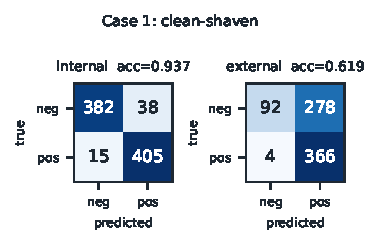
\includegraphics[width=0.315\textwidth]{figures/case1_confusion.pdf}\hfill
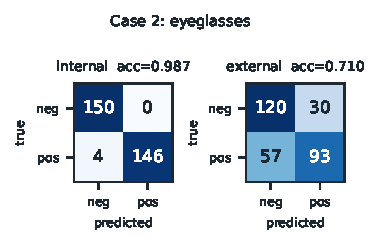
\includegraphics[width=0.315\textwidth]{figures/case2_confusion.pdf}\hfill
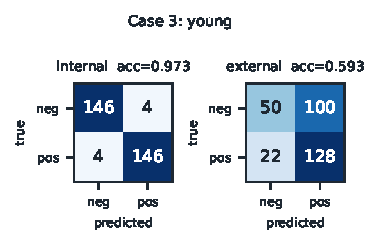
\includegraphics[width=0.315\textwidth]{figures/case3_confusion.pdf}
\end{center}
\vspace{-4pt}
\begin{quote}
\small\textbf{Figure 1.} Confusion matrices on both splits of each case, counts shown. The three
failures have different shapes: case 1 floods false positives (278 externally, 38
internally), case 2 misses 57 positives while making only 30 false positives, and case 3
errs on both sides while staying confident.
\end{quote}
\vspace{2pt}
}]

Three ResNet-18 classifiers, each built by a different team for a different CelebA attribute,
passed internal testing and then failed in deployment. Each was reloaded unchanged and evaluated on
its supplied splits, with no retraining anywhere. Every case ran the same battery: the image
statistics of all four class folders before any prediction was made, then confusion matrices,
precision, recall and F1, ROC and AUC for discrimination, a ten-bin reliability diagram with
expected calibration error, the accuracy of the most confident predictions, and class activation
maps. Each case then ran one further experiment, designed so that a negative result would have
falsified its diagnosis. Aggregate accuracy cannot separate the three faults, since all three land
in a similar band externally (Table~1); the other axes are what distinguish them.

% Declared this early on purpose. A figure* can only be placed at the top of a page at or after
% its declaration point, so declaring it beside the text that discusses it leaves it no page top to
% claim and LaTeX defers it to a float page of its own, which would be a third page and a zero.
% Figure 1 is hand-set inside \twocolumn[...] and is not a float, so the float counter has never
% been advanced. Without this the caption below prints as "Figure 1" while every cross-reference
% in the text says Figure 2.
\setcounter{figure}{1}
\begin{figure*}[t]
\centering
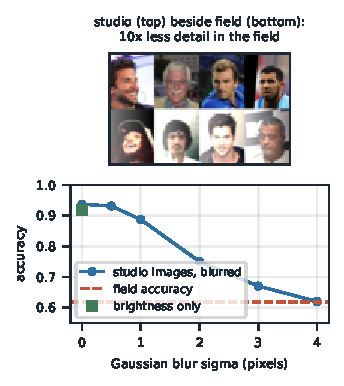
\includegraphics[height=5.9cm]{figures/case1_evidence.pdf}\hfill
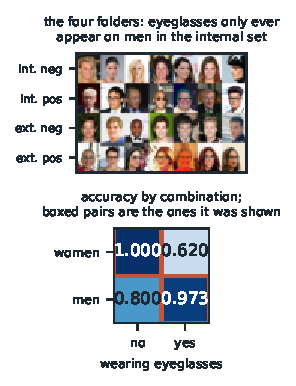
\includegraphics[height=5.9cm]{figures/case2_evidence.pdf}\hfill
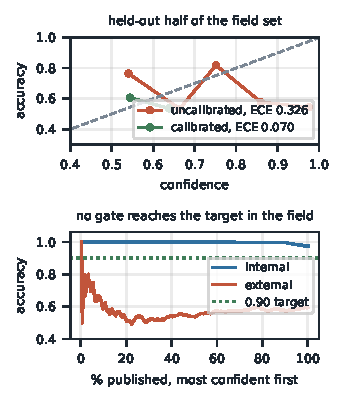
\includegraphics[height=5.9cm]{figures/case3_evidence.pdf}
\caption{The experiment that identifies each fault. \textbf{Left, case 1:} field images beside
studio ones, and the accuracy of the studio set as blur is swept across it; blur alone reaches the
field result, the brightness shift does not. \textbf{Centre, case 2:} the four class folders, and
accuracy split by attribute combination, with the two combinations the internal set contained
outlined. \textbf{Right, case 3:} calibration measured on a held-out half of the field set, and
accuracy against the fraction published when predictions are ordered by confidence.}
\end{figure*}

\section{Case 1: clean-shaven, studio to mobile}
\textbf{Diagnosis: texture dependency, exposed by a loss of image detail between studio and mobile
capture.} The classifier reads ``clean-shaven'' from fine stubble texture on the chin and jaw. The
mobile images carry a fraction of the detail the studio images do, so that texture is gone and a
face that is not clean-shaven no longer looks different from one that is.

\textbf{Experiments and evidence.} At identical pixel dimensions and file format, the field images have a Laplacian
variance 9.9 times lower than the studio ones, 0.00109 against 0.01077, and are
0.262 brighter. The same measurement on cases 2 and 3 gives ratios of 1.2 and
0.9, so the gap belongs to this case rather than to the way it is measured. The errors are
one-sided in the direction that texture loss predicts: false positives rise from 38 to
278 while recall \emph{rises} to 0.989.

The decisive test blurs the studio images and changes nothing else, so the subjects and the labels
are identical throughout. Accuracy falls monotonically with blur and passes through the field
result: at a Gaussian sigma of 4.0 pixels it reaches 0.620 against the field's
0.619, and arrives with the same shape, 310 false positives against 278
(Figure~2, left). The brightness shift applied on its own reaches only 0.918, so exposure
differs between the splits but does not cause the failure. Gaussian blur is a stand-in for whatever
the mobile pipeline does rather than a claim about it; what the sweep establishes is
that removing detail is sufficient to produce the failure, so a field set of different or harder
subjects is not needed to explain it. Saliency agrees: splitting each activation map into three
bands of the face shows 0.542 of the attention on the mouth and jaw when the model is
right, falling to 0.327 when it is wrong while the forehead and hair share rises from
0.042 to 0.242. Once the texture is gone the region that should
decide the prediction holds nothing to decide it with.

\textbf{Recommendations.} Gate on sharpness at inference. Laplacian variance is one cheap statistic
per frame, and a frame below the studio range should prompt a retake rather than be scored. Match
the pre-processing to the capture path so the model is not asked for detail the camera never
recorded. The real fix is to extend the training data with mobile-quality captures and validate on
a held-out mobile sample, because a detector for a texture cue can only be trusted where the
texture survives.

\section{Case 2: eyeglasses at a retail kiosk}
\textbf{Diagnosis: a spurious correlation between eyeglasses and the subject's sex, learned because
the internal set contains only two of the four possible combinations of the two.}

\textbf{Experiments and evidence.} Displaying all four class folders (Figure~2, centre) shows the internal set is
built from women without eyeglasses and men wearing them, while the external set holds exactly the
two combinations that never appear internally. Eyeglasses and sex are therefore perfectly
confounded in everything the model was validated against, and a classifier responding only to sex
would have reached close to the reported internal accuracy of 0.987 without representing
eyeglasses at all.

Stratifying the same predictions by combination separates the two explanations that aggregate
accuracy conflates. It reaches 0.987 accuracy on the two combinations present
internally and 0.710 on the two absent from it, an error rate 22 times higher. The errors fall
on both sides exactly as a sex cue predicts, missing eyeglasses on 57 of the
150 women wearing them and reporting eyeglasses on 30 men who are not. A model that
had merely degraded would err evenly across subjects; this one errs according to whether the
subject matches the pairing it was trained under, which is precisely the reported symptom of
working for some users and not others on images of equal quality.

Saliency measures the same thing directly. Splitting each activation map into three horizontal
bands of the face shows that on predictions the model gets right, 0.552 of its
attention falls on the eyes and nose, where eyeglasses are. On the ones it gets wrong that share
drops to 0.325 and the largest share, 0.498, moves to the mouth and
jaw. The model looks at the eyeglasses when it succeeds and elsewhere when it fails.

\textbf{Recommendations.} Recalibration cannot help, because the fault is in the representation
rather than in the confidence attached to it. Rebuild the validation set so eyeglasses and sex vary
independently, which means collecting the two missing combinations, and report performance per
combination rather than in aggregate, since an aggregate over an unbalanced set concealed this for
the whole lab phase. Until then the kiosk should confirm with the user rather than act on the
prediction, which costs one tap and avoids a recommendation resting on a demographic inference
nobody specified.

\begin{table}[b]
\centering
\footnotesize
\setlength{\tabcolsep}{3pt}
\begin{tabular}{@{}llrrrrrr@{}}
\toprule
Case & Split & Acc & P & R & F1 & AUC & ECE \\
\midrule
1 clean-shaven & internal & 0.937 & 0.914 & 0.964 & 0.939 & 0.9845 & 0.013 \\
1 clean-shaven & external & 0.619 & 0.568 & 0.989 & 0.722 & 0.8459 & 0.250 \\
2 eyeglasses & internal & 0.987 & 1.000 & 0.973 & 0.986 & 0.9997 & 0.013 \\
2 eyeglasses & external & 0.710 & 0.756 & 0.620 & 0.681 & 0.8125 & 0.152 \\
3 young & internal & 0.973 & 0.973 & 0.973 & 0.973 & 0.9960 & 0.036 \\
3 young & external & 0.593 & 0.561 & 0.853 & 0.677 & 0.5640 & 0.296 \\
\bottomrule
\end{tabular}
\caption{All three cases fall into a similar accuracy band externally. AUC, which measures
discrimination, and ECE, which measures whether the confidence can be believed, are what separate
them: case 1 keeps most of its ranking, case 3 loses nearly all of it, and only case 3 is badly
calibrated internally as well.}
\end{table}


\section{Case 3: ``appears young'' with an auto-publish bypass}
\textbf{Diagnosis: overconfidence under distribution shift.} The model does not transfer to the
deployed population and its confidence does not reveal it; validating on an unrepresentative
internal set is the cause. The internal negatives are clearly elderly faces while the field negatives are
middle-aged, so the lab phase measured a much easier problem than deployment poses.

\textbf{Experiments and evidence.} Internally the model reaches AUC 0.9960 and is reasonably calibrated at ECE
0.036, so the bypass looked safe. Externally AUC falls to 0.5640, close to the 0.5 of a
coin toss: the scores no longer rank the classes. The softmax nevertheless keeps emitting extreme
probabilities, so ECE rises to 0.296. The consequence for the bypass is direct. Of the field
predictions issued at 0.90 confidence or above, 54.3 percent of the split, only
0.558 are correct. Raising the gate to 0.99 leaves 20.0 percent published at
0.517, so tightening it does not help: the confidence that selects them is no longer
informative about whether they are right. Both thresholds are reported because the assessment page
and the supplied notebook state different ones, and the conclusion is the same at either.

Fitting a temperature on half the field set and measuring on the other half confirms the mechanism.
Expected calibration error falls from 0.326 to 0.070 while AUC stays at
0.544, unchanged, because dividing a logit by a constant is monotone and cannot reorder
predictions. The fitted temperature is 12.16, and after scaling the most confident field
image reaches only 0.687, so a gate at either threshold would publish 0 of the
150 held-out images. The risk-coverage curve states the ceiling directly: the best accuracy
reachable at any coverage above two percent of the field split is 0.800 (Figure~2, right).

\textbf{Recommendations.} Switch the bypass off rather than re-tune its threshold. No threshold
publishes at 0.90 accuracy on this population, so any gate setting trades volume against errors
instead of avoiding them. Recalibrate, but treat it as instrumentation rather than a repair: a
calibrated score is what lets monitoring detect this condition, and the fact that almost nothing
then clears the gate is the honest reading, not a defect of the calibration. Rebuild the internal
set so its negatives span the ages the system actually meets, and monitor expected calibration
error and high-confidence accuracy continuously, because both looked healthy in the lab and neither
stayed so.

\section{Summary}
The three models fail at similar accuracy for different reasons, which is why the remedies differ.
Case 1 is a property of the inputs, case 2 of the training distribution, and case 3 of the
validation design. In all three the aggregate metric that passed the lab phase is the same metric
that hid the fault, which is the general lesson: an audit has to compare distributions and stratify
results rather than summarise them.

\end{document}
